When describing rotating p	articles it is common to use the so called Euler angles. A formal definition is given by Weber \emph{et al}~\cite{eulerAngles} but for the purposes of this thesis we will describe it as a transformation from our stationary coordinate system $\{x,y,z\}$ to the coordinate system attached to our particle \{x',y',z'\}. This transformation is performed in three steps by using the intermediate axis T.

\begin{itemize}
\item Rotate the x-y plane $\phi$ about the z-axis.
\item Denote the shifted x axis T and rotate the z-y' plane $\theta$ around this axis
\item Rotate $\psi$ around the z' axis to obtain the final coordinate system
\end{itemize}

This is illustrated in figure \ref{fig:eulerangles} where each prim marks one more step of rotation to the coordinate system. Figure \ref{fig:eulerparticle} shows the Euler angle rotations for a triaxial particle shown from a point of view similar to the of the experiment where the X-Z plane is the primary plane. This means we can describe the orientation of a particle using $\mathbf{E} = (\phi, \theta, \psi)$.


\begin{figure}[H]
\centering
\begin{subfigure}[b]{0.45\textwidth}
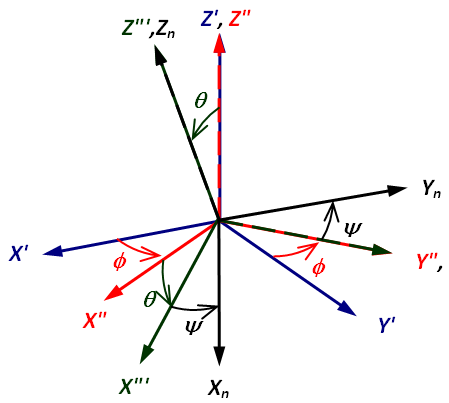
\includegraphics[width=0.9\textwidth]{figures/theory/eulerangles.png}
\caption{A general illustration of Euler angle}
\label{fig:eulerangles}
\end{subfigure}
\begin{subfigure}[b]{0.45\textwidth}
\includegraphics[width=0.9\textwidth]{figures/theory/EulerAngles.pdf}
\caption{The Euler angles as used in our Experiment}
\label{fig:eulerparticle}
\end{subfigure}
\caption{Figure (\subref{fig:eulerangles}) shows the Euler angles illustrated using a series of coordinate rotations. 
Figure (\subref{fig:eulerparticle}) show the Euler angles illustrated using an ellipsoid. This alternate visualization shows the angles with a point of view similar to that of the camera in the experiment. $\psi$ has an impact on the particle dynamics but we can not observe it as the particle is nearly axis-symmetric.}\label{fig:eulerplots}
\end{figure}


%\begin{figure}[H]
%\begin{center}
%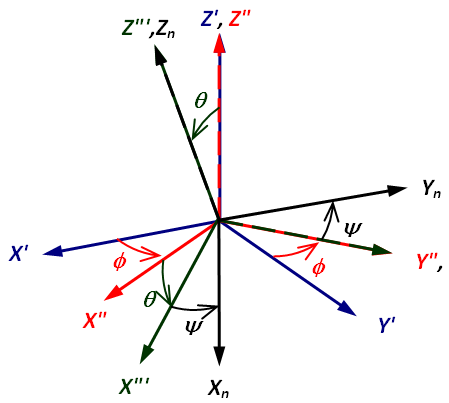
\includegraphics[width=0.6\textwidth]{figures/theory/eulerangles.png}
%\end{center}
%\caption{The Euler angles illustrated using a series of coordinate rotations. This is the normal way of illustrating the Euler angles as it is how they are defined.}
%\label{fig:eulerangles}
%\end{figure}
%
%
%\begin{figure}[H]
%\begin{center}
%\includegraphics[width=0.6\textwidth]{figures/theory/EulerParticle.pdf}
%\end{center}
%\caption{The Euler angles illustrated using an ellipsoid. This alternate visualization shows the angles with a point of view similar to that of the camera in the experiment. Note although $\psi$ has an impact on the particle dynamics, as the particle is nearly axis-symmetric we can not observe it}
%\label{fig:eulerparticle}
%\end{figure}

% Write something about the coordinate system here?

\subsection{Triaxial particles}
Triaxial particles have, as the name suggests, three axis which are all distinct, compared to a sphere which has only one and an ellipse that has two. I will in this thesis refer to the lengths of these axes as $a_x, a_y, a_z$ corresponding to their lengths along those axes for $\mathbf{E} = (0,0,0)$. 

It is, when discussing triaxial particles that are close to being axissymmetric or ellipsoids of the form $a_x \gg a_y \approx a_z$, convenient to introduce the particle asymmetry $\epsilon$ defined as

\begin{equation}\label{eq:epsilon}
\epsilon = \frac{a_y}{a_z} - 1,
\end{equation}

and the aspect ratio $\lambda$ given by

\begin{equation}\label{eq:lambda}
\lambda = \frac{a_x}{a_y}.
\end{equation}


% Where are we talking about this elsehwere?
%When trying to estimate the orientation of the particle from a projection in the x-z plane we will also be interested in the normalized projection of the particle onto the x-z plane. This will be referred to as $\mathbf{n} = (n_x, n_y, n_z)$

%We are interested in the orientation of the particle

%\begin{equation}
%n(t) = (n_x(t), n_y(t), n_z(t))^\intercal.
%\end{equation}

